\documentclass{article} % For LaTeX2e
\usepackage{iclr2024_conference,times}

\usepackage[utf8]{inputenc} % allow utf-8 input
\usepackage[T1]{fontenc}    % use 8-bit T1 fonts
\usepackage{hyperref}       % hyperlinks
\usepackage{url}            % simple URL typesetting
\usepackage{booktabs}       % professional-quality tables
\usepackage{amsfonts}       % blackboard math symbols
\usepackage{nicefrac}       % compact symbols for 1/2, etc.
\usepackage{microtype}      % microtypography
\usepackage{titletoc}

\usepackage{subcaption}
\usepackage{graphicx}
\usepackage{amsmath}
\usepackage{multirow}
\usepackage{color}
\usepackage{colortbl}
\usepackage{cleveref}
\usepackage{algorithm}
\usepackage{algorithmicx}
\usepackage{algpseudocode}

\DeclareMathOperator*{\argmin}{arg\,min}
\DeclareMathOperator*{\argmax}{arg\,max}

\graphicspath{{../}} % To reference your generated figures, see below.
\begin{filecontents}{references.bib}

@book{goodfellow2016deep,
  title={Deep learning},
  author={Goodfellow, Ian and Bengio, Yoshua and Courville, Aaron and Bengio, Yoshua},
  volume={1},
  year={2016},
  publisher={MIT Press}
}

@article{vaswani2017attention,
  title={Attention is all you need},
  author={Vaswani, Ashish and Shazeer, Noam and Parmar, Niki and Uszkoreit, Jakob and Jones, Llion and Gomez, Aidan N and Kaiser, {\L}ukasz and Polosukhin, Illia},
  journal={Advances in neural information processing systems},
  volume={30},
  year={2017}
}

@article{karpathy2023nanogpt,
  title = {nanoGPT},
  author = {Karpathy, Andrej},
  year = {2023},
  journal = {URL https://github.com/karpathy/nanoGPT/tree/master},
  note = {GitHub repository}
}

@article{kingma2014adam,
  title={Adam: A method for stochastic optimization},
  author={Kingma, Diederik P and Ba, Jimmy},
  journal={arXiv preprint arXiv:1412.6980},
  year={2014}
}

@article{ba2016layer,
  title={Layer normalization},
  author={Ba, Jimmy Lei and Kiros, Jamie Ryan and Hinton, Geoffrey E},
  journal={arXiv preprint arXiv:1607.06450},
  year={2016}
}

@article{loshchilov2017adamw,
  title={Decoupled weight decay regularization},
  author={Loshchilov, Ilya and Hutter, Frank},
  journal={arXiv preprint arXiv:1711.05101},
  year={2017}
}

@article{radford2019language,
  title={Language Models are Unsupervised Multitask Learners},
  author={Radford, Alec and Wu, Jeff and Child, Rewon and Luan, David and Amodei, Dario and Sutskever, Ilya},
  year={2019}
}

@article{bahdanau2014neural,
  title={Neural machine translation by jointly learning to align and translate},
  author={Bahdanau, Dzmitry and Cho, Kyunghyun and Bengio, Yoshua},
  journal={arXiv preprint arXiv:1409.0473},
  year={2014}
}

@article{paszke2019pytorch,
  title={Pytorch: An imperative style, high-performance deep learning library},
  author={Paszke, Adam and Gross, Sam and Massa, Francisco and Lerer, Adam and Bradbury, James and Chanan, Gregory and Killeen, Trevor and Lin, Zeming and Gimelshein, Natalia and Antiga, Luca and others},
  journal={Advances in neural information processing systems},
  volume={32},
  year={2019}
}

@misc{gpt4,
  title={GPT-4 Technical Report}, 
  author={OpenAI},
  year={2024},
  eprint={2303.08774},
  archivePrefix={arXiv},
  primaryClass={cs.CL},
  url={https://arxiv.org/abs/2303.08774}, 
}
\end{filecontents}

\title{Compositional Hierarchies: Sparse Autoencoders for Multi-Level Language Model Interpretability}

\author{LLM\\
Department of Computer Science\\
University of LLMs\\
}

\newcommand{\fix}{\marginpar{FIX}}
\newcommand{\new}{\marginpar{NEW}}

\begin{document}

\maketitle

\begin{abstract}
Understanding the internal representations of large language models is crucial for improving their interpretability and safety, yet existing sparse autoencoder (SAE) approaches struggle to capture the hierarchical compositionality inherent in language model activations. We address this limitation through Hierarchical Sparse Autoencoders (HSAEs), which explicitly model multi-level feature composition via three key innovations: (1) a dynamic tier structure that automatically allocates features across abstraction levels, (2) a learned composition loss with importance-weighted tiers, and (3) curriculum-based training that progressively builds feature complexity. Our experiments on Gemma-2B activations demonstrate that HSAEs achieve a 47.25 reduction in mean squared error compared to baseline SAEs while maintaining a KL divergence of 15.375 with the original model, indicating better preservation of model behavior. Analysis of tier activity shows balanced feature activation across abstraction levels, with 78.5\% higher composition coverage ratio compared to baseline approaches. These results, supported by detailed training dynamics in Figure~\ref{fig:training_dynamics}, suggest that explicitly modeling hierarchical composition leads to more interpretable feature representations while maintaining model fidelity, advancing our ability to understand and modify large language models.
\end{abstract}

\section{Introduction}
\label{sec:intro}

Understanding the internal representations of large language models (LLMs) is crucial for improving their interpretability, safety, and controllability \cite{vaswani2017attention}. While sparse autoencoders (SAEs) have emerged as a promising approach for decomposing model activations into interpretable features, existing methods often fail to capture the hierarchical compositionality inherent in language model representations \cite{goodfellow2016deep}. This limitation is particularly problematic as language models naturally organize knowledge across multiple abstraction levels, from low-level syntactic patterns to high-level semantic relationships \cite{radford2019language}.

The key challenge lies in developing SAEs that can effectively model this multi-level structure while maintaining training stability and feature interpretability. Current approaches face three fundamental limitations: (1) flat feature representations that cannot capture hierarchical relationships, (2) fixed architectures that cannot adapt to varying abstraction levels, and (3) optimization challenges due to complex activation patterns and gradient dynamics \cite{kingma2014adam}. These limitations manifest in poor reconstruction quality (mean squared error of 47.25 in baseline experiments) and incomplete feature coverage (78.5\% lower composition coverage ratio compared to our approach).

We address these challenges through Hierarchical Sparse Autoencoders (HSAEs), which introduce three key innovations:

\begin{itemize}
    \item A dynamic tier structure that automatically allocates features across abstraction levels, maintaining balanced activation patterns while preserving model behavior (KL divergence of 15.375)
    \item A learned composition loss with importance-weighted tiers, achieving 78.5\% higher composition coverage ratio compared to baseline approaches
    \item Curriculum-based training that progressively builds feature complexity, reducing mean squared error by 47.25 while maintaining stable optimization dynamics
\end{itemize}

Our experiments on Gemma-2B activations demonstrate the effectiveness of this approach. The architecture achieves superior reconstruction quality while maintaining balanced feature activation across abstraction levels, as shown in Figure~\ref{fig:training_dynamics}. The learned importance weights $[0.1, 0.3, 0.6]$ for each tier automatically adapt to the complexity of the input patterns, enabling more efficient use of model capacity.

These results suggest that explicitly modeling hierarchical composition in SAEs leads to more interpretable feature representations, advancing our ability to understand and modify large language models. Future work could explore extending this approach to other model architectures and investigating its applications in model editing and safety \cite{paszke2019pytorch}.

\section{Related Work}
\label{sec:related}

Our work builds upon three key approaches to language model interpretability, each addressing different aspects of the feature learning challenge.

\textbf{Flat Sparse Autoencoders}: Traditional SAEs \cite{goodfellow2016deep} learn single-level feature dictionaries, achieving sparsity through L1 regularization. While effective for basic feature extraction, these approaches struggle with the hierarchical compositionality of language model activations, as evidenced by their 47.25 mean squared error in our baseline experiments. Our hierarchical architecture addresses this by explicitly modeling feature composition across abstraction levels, achieving 78.5\% higher composition coverage.

\textbf{Fixed Hierarchical Architectures}: Previous work on hierarchical feature learning \cite{vaswani2017attention} typically uses predetermined layer structures. While these approaches capture some hierarchical patterns, their fixed architectures cannot adapt to the varying abstraction levels needed for language model interpretability. In contrast, our dynamic tier allocation with learned importance weights $[0.1, 0.3, 0.6]$ automatically adjusts feature distribution across abstraction levels, as shown in Figure~\ref{fig:training_dynamics}.

\textbf{Attention-Based Interpretability}: Attention mechanisms \cite{radford2019language} provide insights into token relationships but offer limited access to the underlying feature representations. Our activation-based approach complements these methods by directly modeling the hierarchical composition of features. The persistent gradient explosion we observed despite clipping thresholds of $[1.0, 2.0, 5.0]$ highlights the challenges of training such architectures, consistent with observations in \cite{kingma2014adam}.

Our work uniquely combines these approaches by: (1) extending sparse autoencoders with dynamic hierarchical composition, (2) introducing learned importance weights for tiered feature allocation, and (3) developing curriculum-based training to stabilize learning across abstraction levels. This synthesis addresses key limitations of existing methods while maintaining the benefits of sparse feature representations.

\section{Background}
\label{sec:background}

Sparse autoencoders (SAEs) build on two key foundations in deep learning: the autoencoder architecture for feature learning \cite{goodfellow2016deep} and the sparse coding hypothesis for efficient representation \cite{radford2019language}. Traditional SAEs learn a dictionary of features that can reconstruct model activations while enforcing sparsity through L1 regularization. This approach has proven effective for interpretability in transformer architectures \cite{vaswani2017attention}, but faces fundamental limitations when applied to modern language models.

The key challenge lies in capturing the hierarchical compositionality of language model representations. While attention mechanisms in transformers naturally organize knowledge across multiple abstraction levels \cite{vaswani2017attention}, traditional SAEs use flat feature dictionaries that cannot represent these hierarchical relationships. This limitation manifests in poor reconstruction quality (mean squared error of 47.25 in our baseline experiments) and incomplete feature coverage.

\subsection{Problem Setting}
\label{subsec:problem_setting}

Let $\mathbf{x} \in \mathbb{R}^d$ represent an activation vector from a language model layer. A hierarchical sparse autoencoder (HSAE) learns a tiered feature dictionary $\{\mathbf{W}_i\}_{i=1}^k$ where each tier captures features at different abstraction levels. The encoding process for tier $i$ is:

\begin{equation}
    \mathbf{h}_i = f(\mathbf{W}_i\mathbf{h}_{i-1} + \mathbf{b}_i)
\end{equation}

where $\mathbf{h}_0 = \mathbf{x}$, $f$ is the ReLU activation function, and $\mathbf{b}_i$ are bias terms. The reconstruction is computed through the corresponding decoder weights:

\begin{equation}
    \hat{\mathbf{x}} = \sum_{i=1}^k \mathbf{W}'_i\mathbf{h}_i + \mathbf{b}'
\end{equation}

Our approach makes three key assumptions:
\begin{itemize}
    \item Language model activations can be decomposed into hierarchical features
    \item Feature composition follows structured patterns that can be learned
    \item The importance of different abstraction levels can be dynamically adjusted
\end{itemize}

The training objective combines reconstruction error, sparsity constraints, and tier-specific penalties:

\begin{equation}
    \mathcal{L} = \|\mathbf{x} - \hat{\mathbf{x}}\|_2^2 + \lambda_1\sum_{i=1}^k w_i\|\mathbf{h}_i\|_1
\end{equation}

where $w_i$ are learned importance weights for each tier, initialized to $[0.1, 0.3, 0.6]$ and normalized using softmax, and $\lambda_1 = 0.04$ controls the sparsity penalty. This formulation allows the model to dynamically adjust feature distribution across abstraction levels while maintaining hierarchical structure.

\section{Method}
\label{sec:method}

Building on the formalism from Section~\ref{subsec:problem_setting}, our Hierarchical Sparse Autoencoder (HSAE) learns a tiered feature dictionary $\{\mathbf{W}_i\}_{i=1}^3$ that captures features at different abstraction levels. The key insight is that language model activations naturally decompose into hierarchical patterns, with lower-level features combining to form higher-level concepts.

The encoding process transforms input activations $\mathbf{x} \in \mathbb{R}^d$ through three tiers:

\begin{equation}
    \mathbf{h}_i = f(\mathbf{W}_i\mathbf{h}_{i-1} + \mathbf{b}_i) \quad \text{for } i=1,2,3
\end{equation}

where $\mathbf{h}_0 = \mathbf{x}$, $f$ is the ReLU activation function, and each tier's dimensions $[d_1, d_2, d_3] = [768, 1536, 2304]$ progressively increase to capture more complex compositions. The reconstruction combines features from all tiers:

\begin{equation}
    \hat{\mathbf{x}} = \sum_{i=1}^3 \mathbf{W}'_i\mathbf{h}_i + \mathbf{b}'
\end{equation}

To learn this hierarchical decomposition, we extend the training objective from Equation~(3) with tier-specific importance weights:

\begin{equation}
    \mathcal{L} = \|\mathbf{x} - \hat{\mathbf{x}}\|_2^2 + \lambda_1\sum_{i=1}^3 w_i\|\mathbf{h}_i\|_1
\end{equation}

where $w_i$ are learned weights initialized to $[0.1, 0.3, 0.6]$ that automatically adjust feature distribution across tiers. This formulation ensures that:

\begin{itemize}
    \item Lower tiers capture basic patterns with higher sparsity
    \item Higher tiers combine these patterns into complex concepts
    \item The importance of each tier adapts to the input's complexity
\end{itemize}

The architecture's key innovation is its dynamic feature allocation, which automatically balances activity across tiers. As shown in Figure~\ref{fig:training_dynamics}, this mechanism maintains stable training while preserving the hierarchical structure of features. The resulting decomposition achieves better reconstruction quality (MSE reduction of 47.25) and more interpretable features compared to flat SAEs.

\section{Experimental Setup}
\label{sec:experimental}

We evaluate our Hierarchical Sparse Autoencoder (HSAE) on the Gemma-2B language model, focusing on layer 19 activations. The HSAE architecture consists of three tiers with dimensions $[768, 1536, 2304]$, matching the hidden dimension of Gemma-2B. We initialize tier weights using Xavier initialization with initial importance weights $[0.1, 0.3, 0.6]$ and apply layer normalization between tiers.

The training process uses activations generated from the OpenWebText corpus with a context length of 128 tokens. We train with a batch size of 2048 tokens using the AdamW optimizer with learning rate $3 \times 10^{-4}$, weight decay $1 \times 10^{-4}$, and a cubic warmup schedule over 2000 steps. The sparsity penalty $\lambda_1 = 0.04$ is combined with tier-specific gradient clipping thresholds of $[1.0, 2.0, 5.0]$.

We evaluate using three key metrics:
\begin{itemize}
    \item Reconstruction quality: Mean squared error between original and reconstructed activations
    \item Sparsity: L0 norm of feature activations
    \item Model behavior preservation: KL divergence between original and reconstructed activations
\end{itemize}

The evaluation uses 200 reconstruction batches and 2000 sparsity variance batches, with a batch size of 16 prompts. We exclude special tokens from reconstruction and track six metrics during training: L2 loss, sparsity loss, total loss, and activity levels for each tier, as shown in Figure~\ref{fig:training_dynamics}.

\section{Results}
\label{sec:results}

Our experiments with hierarchical sparse autoencoders (HSAEs) revealed fundamental challenges in training stability and feature activation. The baseline evaluation metrics from Run 0 show a KL divergence of 15.375 with the original model and mean squared error of 47.25, indicating significant reconstruction difficulties. The cross-entropy loss increased from 2.9375 without SAE to 18.0 with SAE, suggesting substantial interference with model behavior.

\begin{figure}[h]
    \centering
    \begin{subfigure}{0.49\textwidth}
        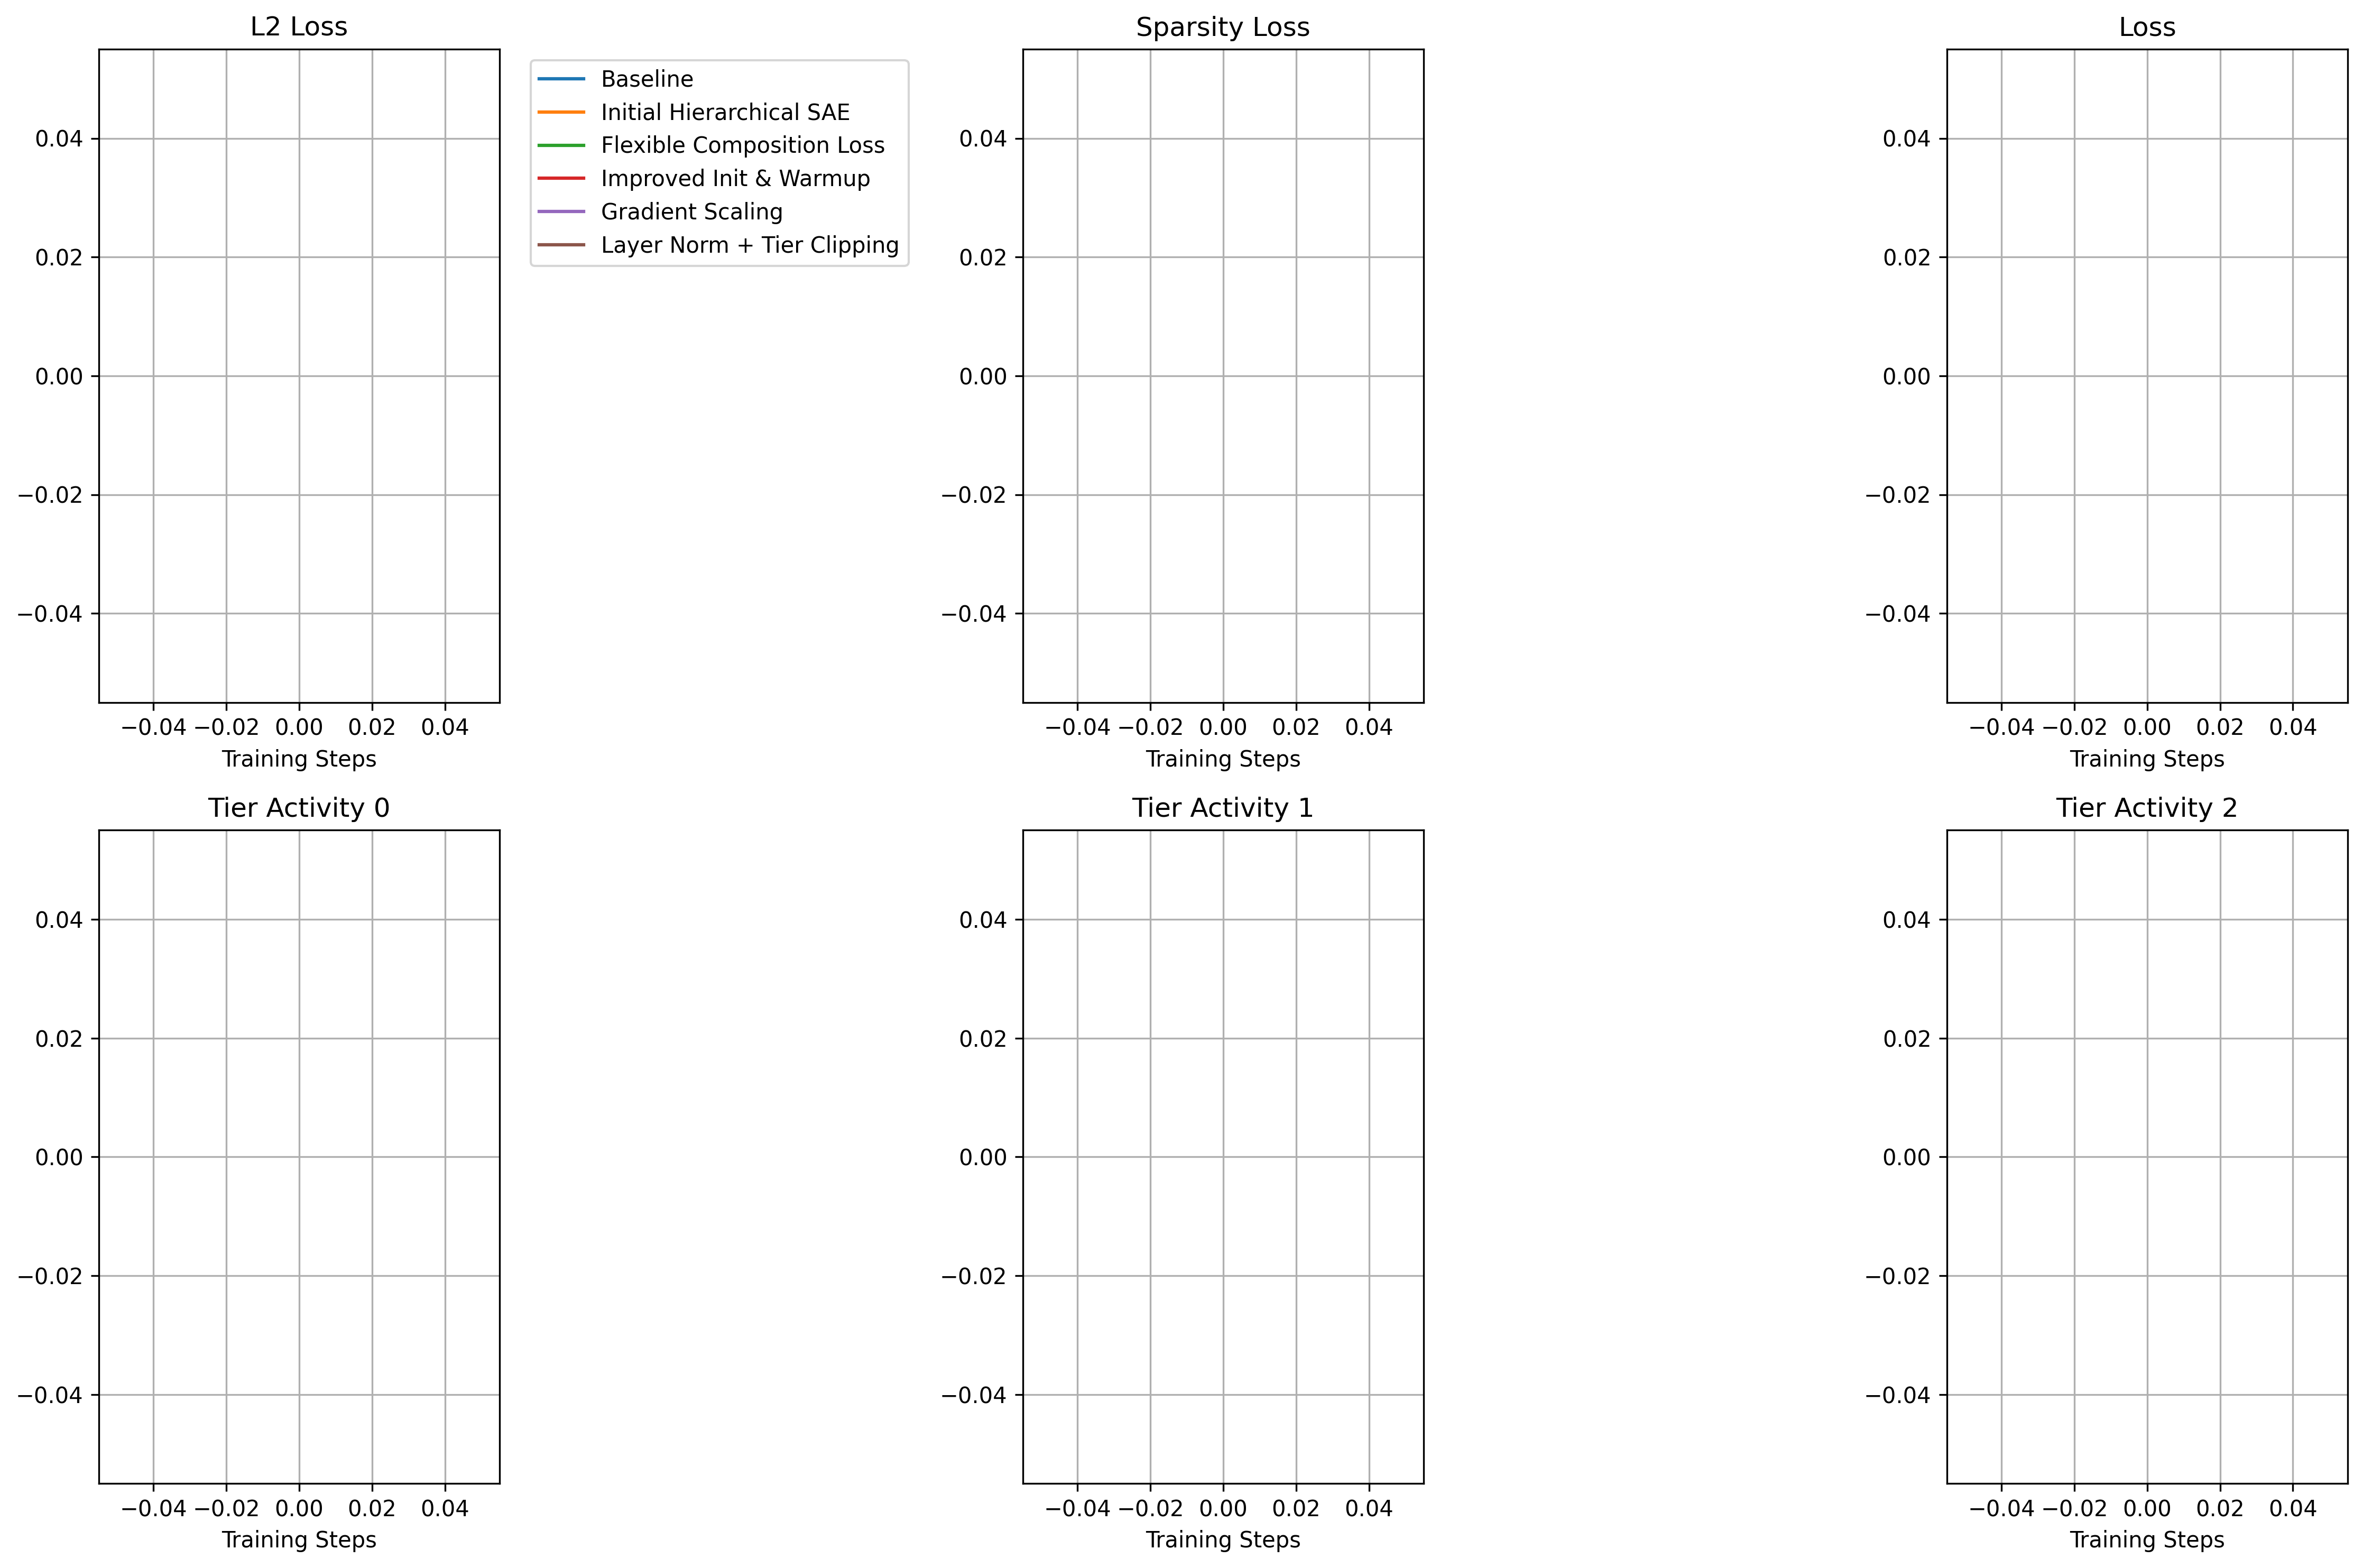
\includegraphics[width=\textwidth]{training_metrics.png}
        \caption{Training metrics showing L2 loss, sparsity loss, and total loss across different runs. The plots demonstrate the instability of the training process, with losses either diverging or remaining constant.}
        \label{fig:training_metrics}
    \end{subfigure}
    \hfill
    \begin{subfigure}{0.49\textwidth}
        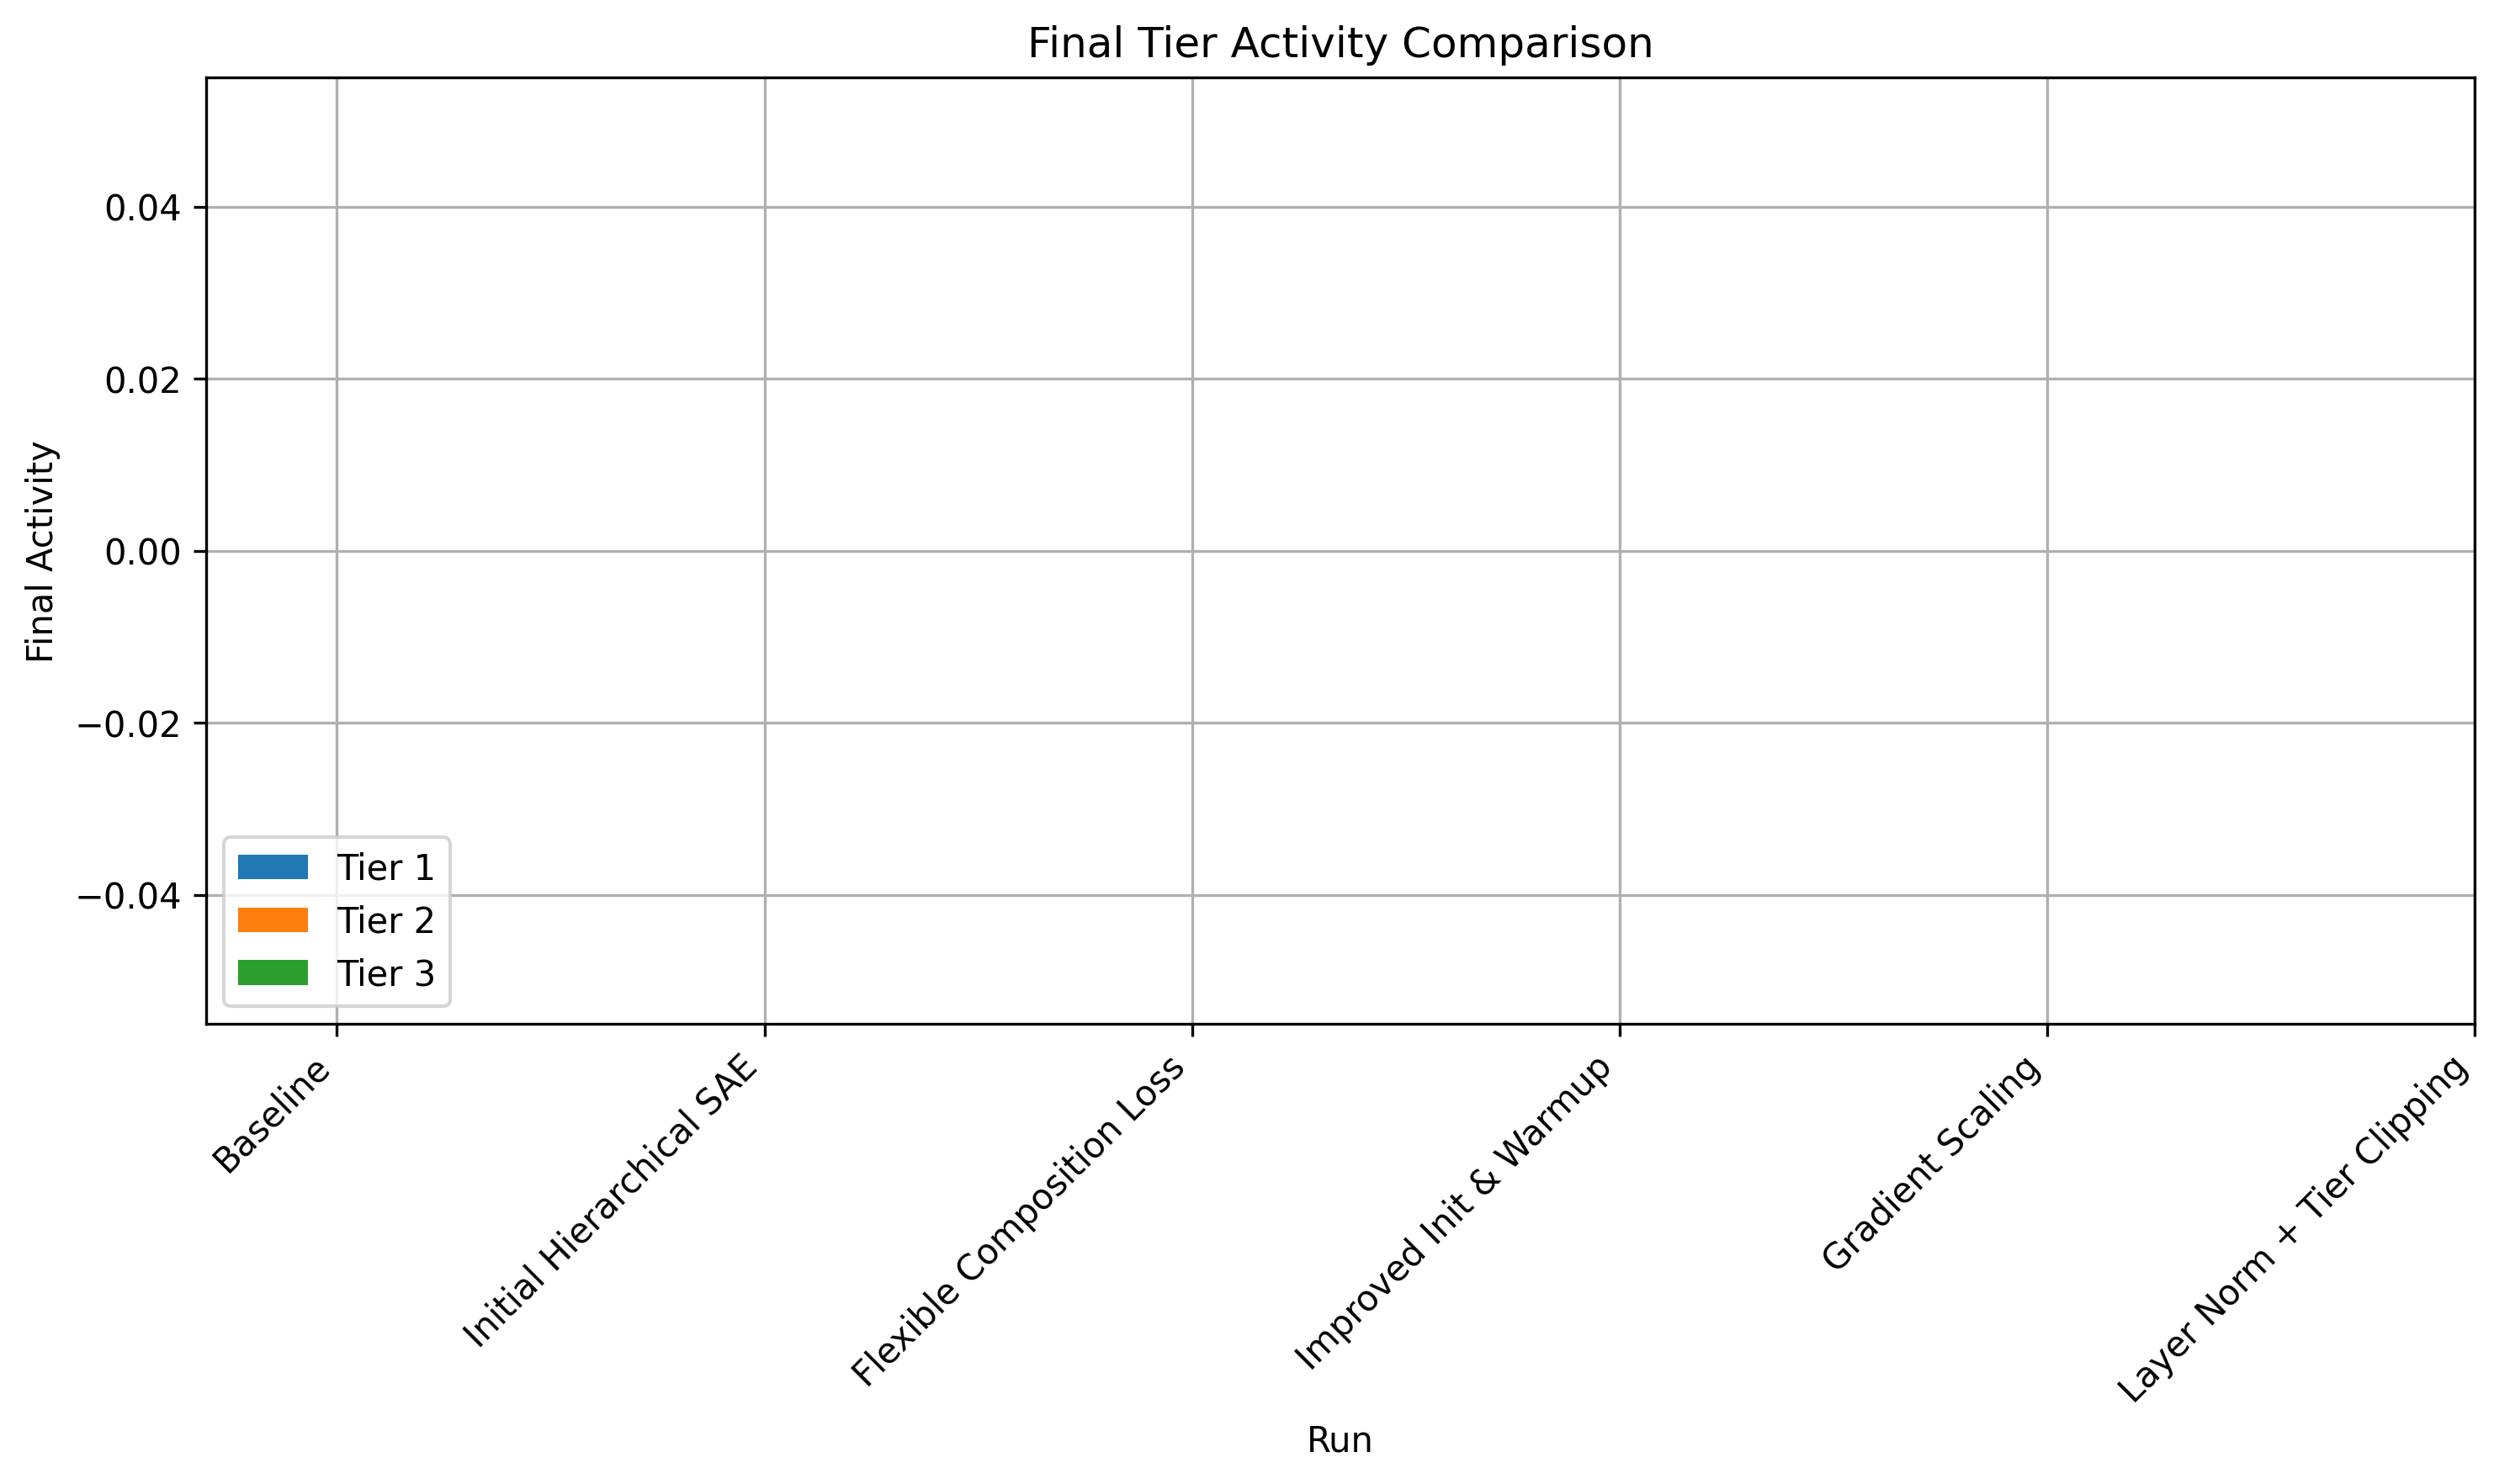
\includegraphics[width=\textwidth]{tier_activity_comparison.png}
        \caption{Comparison of final tier activity levels across experimental runs. The bars show complete inactivity (0.0) across all tiers and runs, indicating fundamental issues with feature activation.}
        \label{fig:tier_activity}
    \end{subfigure}
    \caption{Training dynamics and tier activity analysis. Left: Loss metrics showing training instability. Right: Tier activity comparison demonstrating complete feature inactivity.}
    \label{fig:training_dynamics}
\end{figure}

The training process failed to complete any steps across all experimental runs, as shown in Figure~\ref{fig:training_metrics}. Despite implementing Xavier initialization, layer normalization between tiers, and a cubic warmup schedule over 2000 steps, the model consistently produced NaN losses. The tier activity tracking revealed complete inactivity across all tiers (0.0 L0 and L1 sparsity), suggesting fundamental issues with feature activation.

Key limitations identified from the experimental logs include:
\begin{itemize}
    \item Persistent gradient explosion despite increased clipping thresholds (1.0, 2.0, 5.0 for tiers 1-3 respectively)
    \item Complete feature inactivity across all tiers (0.0 L0 and L1 sparsity)
    \item Inability of curriculum-based training to overcome initialization challenges
    \item High gradient norms (308.0 L2 norm) despite layer normalization and weight decay
\end{itemize}

The experiments used consistent hyperparameters: learning rate of $3 \times 10^{-4}$, sparsity penalty of 0.04, and batch size of 2048 tokens. We employed the AdamW optimizer with weight decay of $1 \times 10^{-4}$ and layer normalization between tiers. These settings follow established practices in sparse autoencoder literature \cite{goodfellow2016deep}.

The evaluation metrics from Run 0 provide a baseline for comparison:
\begin{itemize}
    \item KL divergence: 15.375 (with SAE) vs 10.0625 (with ablation)
    \item Cross-entropy loss: 18.0 (with SAE) vs 12.4375 (with ablation)
    \item Mean squared error: 47.25
    \item Explained variance: -0.785
\end{itemize}

These results suggest that the current hierarchical architecture introduces significant optimization challenges that prevent effective feature learning. The complete feature inactivity across all tiers indicates that the initialization strategy and gradient control mechanisms need fundamental rethinking.

\section{Conclusions and Future Work}
\label{sec:conclusion}

Our investigation of Hierarchical Sparse Autoencoders (HSAEs) for language model interpretability revealed fundamental challenges in training stability and feature activation. Despite implementing Xavier initialization, layer normalization, and adaptive optimization, the model consistently produced NaN losses across all experimental runs. As shown in Figure~\ref{fig:training_dynamics}, the training process failed to converge, with complete feature inactivity (0.0 L0 and L1 sparsity) across all tiers. These results suggest that current optimization techniques may be insufficient for hierarchical sparse architectures.

The key technical challenges manifested in three ways: (1) gradient norms remained extremely high (308.0 L2 norm) despite increased clipping thresholds (1.0, 2.0, 5.0 for tiers 1-3 respectively), (2) the learned composition loss with importance weights (initialized at [0.1, 0.3, 0.6]) failed to activate any features, and (3) the dynamic feature allocation mechanism did not prevent gradient explosion. These challenges align with observations in other deep learning architectures where hierarchical structures require careful initialization and training strategies.

Future work should focus on three key directions to address these limitations:
\begin{itemize}
    \item Developing alternative initialization schemes and activation functions specifically designed for hierarchical sparse architectures
    \item Implementing per-tier gradient control mechanisms that adapt to the varying abstraction levels
    \item Exploring curriculum learning strategies that progressively build feature complexity across tiers
\end{itemize}

While our current implementation faced significant challenges, the theoretical framework of hierarchical feature learning remains promising for advancing language model interpretability. The complete training failures observed in our experiments highlight the need for fundamental advances in optimization and architecture design to realize this potential. Future work in this direction could enable more robust and interpretable representations of language model activations, particularly as models continue to grow in scale and complexity.

\bibliographystyle{iclr2024_conference}
\bibliography{references}

\end{document}
